% =====================================================================
%  Proyecto final — Matemáticas Discretas (MAT 4021), Universidad del Norte
%  Predicción de brotes de dengue en el Atlántico con un grafo de
%  municipios y una red neuronal.
%
%  Compilar:  pdflatex main  (dos veces, para las referencias cruzadas)
%  En Overleaf compila tal cual. Las referencias están escritas en
%  formato APA 7 dentro del mismo archivo (no requiere biber/bibtex).
% =====================================================================
\documentclass[11pt,letterpaper]{article}

\usepackage[T1]{fontenc}
\usepackage[utf8]{inputenc}
\usepackage{lmodern}
\IfFileExists{spanish.ldf}{%
  \usepackage[spanish,es-tabla,es-nodecimaldot]{babel}%
}{%
  % Si babel-spanish no está instalado, al menos los nombres van en español
  \renewcommand{\figurename}{Figura}\renewcommand{\tablename}{Tabla}%
  \renewcommand{\refname}{Referencias}\renewcommand{\contentsname}{Contenido}%
  \renewcommand{\appendixname}{Apéndice}\renewcommand{\abstractname}{Resumen}%
}
\usepackage[margin=2.54cm]{geometry}
\usepackage{setspace}\setstretch{1.15}
\usepackage{amsmath,amssymb}
\usepackage{graphicx}
\usepackage{booktabs,tabularx,multirow}
\usepackage{float}
\usepackage[font=small,labelfont=bf,justification=raggedright,singlelinecheck=false]{caption}
\usepackage{enumitem}\setlist{itemsep=1pt,topsep=3pt}
\usepackage{xcolor}
\usepackage[spanish,ruled,vlined,linesnumbered]{algorithm2e}
\usepackage[round,sort]{natbib}
\IfFileExists{xurl.sty}{\usepackage{xurl}}{}
\usepackage[colorlinks=true,linkcolor=black,citecolor=blue!50!black,urlcolor=blue!50!black]{hyperref}
\usepackage{fancyhdr}
\pagestyle{fancy}\fancyhf{}\fancyhead[R]{\thepage}\renewcommand{\headrulewidth}{0pt}

\newcommand{\inc}{\mathrm{inc}}
\setlength{\parindent}{1.27cm}

% ---------------------------------------------------------------------
\begin{document}

% ======================== PORTADA (formato APA 7, estudiante) ========
\begin{titlepage}
\centering
\vspace*{3.5cm}
{\large\bfseries Predicción de brotes de dengue en los municipios del Atlántico\\[2pt]
con un grafo de municipios vecinos y una red neuronal\par}
\vspace{2cm}
{Samuel Castañeda\\
{[Integrante 2]}\\
{[Integrante 3]}\\
{[Integrante 4]}\par}
\vspace{1cm}
{Departamento de Matemáticas y Estadística, Universidad del Norte\par}
\vspace{0.4cm}
{MAT 4021: Matemáticas Discretas — Grupo 4\par}
\vspace{0.4cm}
{MSc. Iván Gómez\par}
\vspace{0.4cm}
{15 de noviembre de 2026\par}
\end{titlepage}

% ======================== RESUMEN ===================================
\begin{center}{\bfseries Resumen}\end{center}
\noindent
El dengue es endémico en el departamento del Atlántico, donde se notificaron 49.308 casos entre 2018 y 2025. Este trabajo modela el problema con dos herramientas del curso. La primera es un grafo no dirigido cuyos 23 vértices son los municipios y cuyas 47 aristas unen municipios que comparten frontera; las aristas se ponderan con un modelo de gravedad poblacional. La segunda es un perceptrón multicapa que predice si cada municipio tendrá un brote en el siguiente periodo epidemiológico de cuatro semanas. La red recibe la incidencia reciente, la lluvia rezagada y la \emph{presión de los vecinos}, una variable que el grafo calcula. Se usaron datos reales del SIVIGILA, el DANE y Open-Meteo, y algoritmos implementados por el grupo (BFS y el algoritmo de Brandes), verificados a mano y contra la librería NetworkX. En el año de prueba (2025), la red detectó el 88\,\% de los brotes, frente al 68\,\% de una regla de persistencia, con un AUC-ROC de 0,83 frente a 0,77. Sin embargo, la red no superó a una regresión logística, y añadir la presión de los vecinos no mejoró la predicción: la diferencia fue $-0{,}005 \pm 0{,}031$ en AUC-PR sobre 20 semillas. El grafo sí resultó útil para decidir: la intermediación identifica a Sabanalarga y Baranoa como los puentes del contagio entre el área metropolitana y el sur del departamento. Por eso se propone un ranking de fumigación que combina la probabilidad de brote con la centralidad.

\medskip\noindent
\emph{Palabras clave:} dengue, teoría de grafos, centralidad de intermediación, redes neuronales, vigilancia epidemiológica, Atlántico.

\newpage
% ======================== 1. INTRODUCCIÓN ===========================
\section{Introducción}

El dengue es una infección viral transmitida por el mosquito \emph{Aedes aegypti}. No tiene tratamiento específico, y sus formas graves pueden ser mortales, en especial en niños \citep{oms_dengue}. En el Atlántico es un problema recurrente. En 2024 se notificaron 4.226 casos probables hasta el 7 de septiembre \citep{eltiempo2024}. A la semana 19 de 2026 iban 3.441 casos notificados y 12 municipios en declaratoria de brote tipo I \citep{eluniversal2026}.

Las autoridades responden con fumigación y eliminación de criaderos, pero esos recursos son limitados. La pregunta práctica que guía este proyecto es: \emph{¿en qué municipios conviene intervenir primero en el siguiente periodo?} Responderla requiere anticipar los brotes, no solo reaccionar a ellos. También requiere tener en cuenta que el contagio no respeta los límites municipales: las personas se mueven entre municipios vecinos, y con ellas el virus.

\subsection{Por qué es un problema de impacto}

\begin{table}[H]
\centering\small
\caption{El problema frente a las cuatro condiciones de impacto del proyecto.}
\label{tab:impacto}
\begin{tabularx}{\textwidth}{@{}lX@{}}
\toprule
Condición & Respuesta \\
\midrule
Afecta a alguien & Los 2,87 millones de habitantes de los 23 municipios del Atlántico \citep{dane_pob}. Entre 2018 y 2025 hubo 49.308 casos notificados; el 56\,\% en Barranquilla y el 20\,\% en Soledad. \\
Hay evidencia & Microdatos oficiales del SIVIGILA \citep{sivigila}, boletines del Instituto Nacional de Salud y declaratorias de brote de la Gobernación \citep{eluniversal2026}. \\
Se puede mejorar & Se mide qué fracción de los brotes reales se detecta un periodo antes (sensibilidad) y cuántas alertas son correctas (precisión), comparando con la regla actual implícita: ``si hay brote, seguirá habiendo''. \\
Se puede modelar & Grafo ponderado de municipios (vecindad, gravedad, centralidad) y red neuronal (perceptrón multicapa) para clasificar brote / no brote. \\
\bottomrule
\end{tabularx}
\end{table}

\subsection{Objetivos}
\textbf{General.} Construir y evaluar un sistema que anticipe los brotes de dengue en los municipios del Atlántico con un periodo epidemiológico de anticipación, y que priorice la intervención usando la estructura de vecindad entre municipios.

\noindent\textbf{Específicos.}
\begin{enumerate}[label=\arabic*.]
  \item Modelar los municipios como un grafo ponderado y calcular sus medidas de centralidad con algoritmos propios.
  \item Entrenar una red neuronal que prediga el brote del periodo siguiente y compararla con modelos de referencia.
  \item Medir si la información del grafo (presión de los vecinos) mejora la predicción.
  \item Proponer un ranking de prioridad de fumigación que combine riesgo y centralidad.
\end{enumerate}

% ======================== 2. MODELACIÓN =============================
\section{Modelación con la teoría del curso}

\subsection{Datos}
Todos los datos son reales y públicos (Tabla~\ref{tab:datos}). La unidad de tiempo es el \emph{periodo epidemiológico} del Instituto Nacional de Salud: cuatro semanas, trece por año. Con semanas sueltas, el 66\,\% de las combinaciones municipio–semana tenían cero casos. Con periodos de cuatro semanas, esa proporción baja al 35\,\%.

\begin{table}[H]
\centering\small
\caption{Fuentes de datos.}
\label{tab:datos}
\begin{tabularx}{\textwidth}{@{}lXr@{}}
\toprule
Dato & Fuente y procesamiento & Tamaño \\
\midrule
Casos de dengue & SIVIGILA, evento 210, 2018--2025 \citep{sivigila}. Filtro: departamento de ocurrencia = Atlántico (código 08). Cada caso se ubica en la semana de \emph{inicio de síntomas}. & 49.308 casos \\
Población & Proyecciones municipales del DANE, actualización post-COVID \citep{dane_pob}. & 23 × 8 años \\
Límites municipales & Marco Geoestadístico Nacional 2018 \citep{dane_mgn}. & 23 polígonos \\
Coordenadas & Cabeceras municipales, DIVIPOLA \citep{dane_divipola}. & 23 puntos \\
Clima diario & Open-Meteo, modelo ECMWF IFS de 9 km \citep{openmeteo}: lluvia, temperatura y humedad. & 67.206 días \\
\bottomrule
\end{tabularx}
\end{table}

\noindent Resultado: un panel de $23 \times 13 \times 8 = 2.392$ filas (municipio, periodo), con casos, incidencia por cien mil habitantes y clima.

\subsection{El grafo de municipios}
Se define el grafo no dirigido y ponderado $G=(V,E,w)$:
\begin{itemize}
  \item $V$: los 23 municipios del Atlántico.
  \item $\{a,b\}\in E$ si los polígonos de $a$ y $b$ comparten al menos 1\,km de frontera. De 51 contactos entre polígonos, 4 medían menos de 300\,m: son esquinas o artefactos de la cartografía y se descartaron. El siguiente contacto más corto mide 2,1\,km. Quedan $|E| = 47$ aristas y el grafo es conexo.
  \item Peso de gravedad \citep{xia2004}, inspirado en la ley de Newton. La interacción entre dos poblaciones crece con su tamaño y decrece con la distancia:
  \begin{equation}
    w(a,b) = \frac{P_a\,P_b}{d(a,b)^2}\Big/\max_{\{u,v\}\in E}\frac{P_u\,P_v}{d(u,v)^2},
  \end{equation}
  donde $P$ es la población promedio de los años de entrenamiento y $d$ es la distancia en kilómetros entre cabeceras (fórmula de haversine). La arista más pesada es Barranquilla–Soledad ($w=1$).
\end{itemize}

\paragraph{Medidas de centralidad.} Todas son topológicas: cuentan saltos entre vecinos, sin pesos. Sea $d_G(u,v)$ la distancia (número de aristas) del camino más corto entre $u$ y $v$, y sea $n=|V|$.
\begin{align}
  \text{Grado:}\quad & g(v) = |\{u : \{u,v\}\in E\}| \\
  \text{Cercanía:}\quad & C(v) = \frac{n-1}{\sum_{u\neq v} d_G(v,u)} \\
  \text{Intermediación:}\quad & B(v) = \sum_{\{s,t\},\; s\neq v\neq t} \frac{\sigma_{st}(v)}{\sigma_{st}}
\end{align}
donde $\sigma_{st}$ es el número de caminos más cortos entre $s$ y $t$, y $\sigma_{st}(v)$ el número de esos caminos que pasan por $v$ \citep{freeman1977}. La intermediación mide cuánto ``puente'' es un municipio: si se fumiga un municipio con $B(v)$ alta, se cortan muchas rutas de contagio entre otros municipios. La versión normalizada divide entre $(n-1)(n-2)/2$.

\paragraph{Presión de los vecinos.} Es la variable que conecta el grafo con la red neuronal: el promedio de la incidencia de los vecinos, ponderado por la gravedad.
\begin{equation}
  \mathrm{PV}_v(t) = \frac{\sum_{u:\{u,v\}\in E} w(u,v)\,\inc_u(t)}{\sum_{u:\{u,v\}\in E} w(u,v)}.
\end{equation}

\subsection{Definición de brote}
Para el municipio $m$ y el periodo del año $p$, sean $\mu_{m,p}$ y $s_{m,p}$ la media y la desviación estándar de la incidencia en los años de entrenamiento. Se dice que hay brote en el periodo $t$ si
\begin{equation}
  \inc_m(t) > \mu_{m,p(t)} + s_{m,p(t)} \quad\text{y}\quad \text{casos}_m(t) \ge 3 .
\end{equation}
La segunda condición evita que pasar de 0 a 1 caso cuente como brote en un municipio pequeño.

\subsection{La red neuronal}
Se usa un perceptrón multicapa \citep{goodfellow2016}. Cada fila es un municipio $m$ al final del periodo $t$, y el objetivo es $y\in\{0,1\}$: ¿habrá brote en $t+1$? La entrada $\mathbf{x}\in\mathbb{R}^{14}$ contiene:
\begin{itemize}
  \item la incidencia en $t$, $t-1$ y $t-2$, en escala $\log(1+x)$;
  \item la anomalía de lluvia en $t$, $t-1$, $t-2$ y $t-3$, es decir, la lluvia menos el promedio de ese periodo en los años de entrenamiento;
  \item la temperatura y la humedad en $t$;
  \item el periodo del año en forma circular ($\sin$, $\cos$);
  \item el logaritmo de la población;
  \item \textbf{la presión de los vecinos en $t$ y $t-1$}, que es el aporte del grafo.
\end{itemize}
La arquitectura es $14 \to 16 \to 8 \to 1$:
\begin{equation}
  \mathbf{h}_1=\mathrm{ReLU}(W_1\mathbf{x}+\mathbf{b}_1),\quad
  \mathbf{h}_2=\mathrm{ReLU}(W_2\mathbf{h}_1+\mathbf{b}_2),\quad
  \hat y=\sigma(\mathbf{w}_3^\top\mathbf{h}_2+b_3),
\end{equation}
con $\mathrm{ReLU}(z)=\max(0,z)$ y $\sigma(z)=1/(1+e^{-z})$. Los pesos se ajustan minimizando la entropía cruzada con regularización $L_2$,
\begin{equation}
  \mathcal{L} = -\frac{1}{N}\sum_{i=1}^N \big[y_i\log\hat y_i + (1-y_i)\log(1-\hat y_i)\big] + \alpha\lVert W\rVert_2^2,
  \qquad \alpha = 0{,}01,
\end{equation}
mediante retropropagación y el optimizador Adam, con parada temprana \citep{pedregosa2011}. La red predice $\hat y\in(0,1)$, y se emite una alerta cuando $\hat y$ supera un umbral $\tau$ (Sección~\ref{sec:decisiones}).

% ======================== 3. SOLUCIÓN ===============================
\section{Solución: algoritmos y datos}

\subsection{Algoritmos implementados}
Los algoritmos del grafo se programaron sin librerías de grafos (archivo \texttt{src/grafo\_lib.py}). El grafo se guarda como lista de adyacencia. Las distancias $d_G$ se calculan con búsqueda en anchura (BFS) desde cada vértice, en tiempo $O(n+|E|)$ por vértice. La intermediación usa el algoritmo de \citet{brandes2001}, que evita enumerar todos los caminos: por cada origen $s$, un BFS cuenta los caminos más cortos $\sigma_{sv}$ y luego acumula las dependencias en orden inverso de distancia. El costo total es $O(n\,|E|)$.

\begin{algorithm}[H]
\caption{Intermediación de Brandes (grafo no dirigido, sin pesos)}
\SetKwInOut{Entrada}{Entrada}\SetKwInOut{Salida}{Salida}
\Entrada{lista de adyacencia de $G=(V,E)$}
\Salida{$B(v)$ para todo $v\in V$}
$B(v)\leftarrow 0$ para todo $v$\;
\ForEach{$s\in V$}{
  $\sigma(s)\leftarrow1$; $\sigma(v)\leftarrow 0$ y $\mathit{dist}(v)\leftarrow -1$ para $v\neq s$; $\mathit{dist}(s)\leftarrow 0$\;
  BFS desde $s$: al ver la arista $(v,w)$ con $\mathit{dist}(w)=\mathit{dist}(v)+1$, hacer $\sigma(w)\mathrel{+}=\sigma(v)$ y añadir $v$ a $\mathit{pred}(w)$; apilar cada $v$ visitado\;
  $\delta(v)\leftarrow0$ para todo $v$\;
  \While{la pila no esté vacía}{
    $w\leftarrow$ desapilar\;
    \lForEach{$v\in\mathit{pred}(w)$}{$\delta(v)\mathrel{+}=\frac{\sigma(v)}{\sigma(w)}\,(1+\delta(w))$}
    \lIf{$w\neq s$}{$B(w)\mathrel{+}=\delta(w)$}
  }
}
\Return $B(v)/2$ para todo $v$ \tcp*{cada par se contó dos veces}
\end{algorithm}

\subsection{Flujo de datos}
El ejecutable consta de siete scripts de Python que se corren en orden (Tabla~\ref{tab:scripts}). Las instrucciones están en el archivo \texttt{README.md}.

\begin{table}[H]
\centering\small
\caption{Programas del proyecto.}
\label{tab:scripts}
\begin{tabularx}{\textwidth}{@{}lX@{}}
\toprule
Script & Función \\
\midrule
\texttt{01\_casos.py} & Semana epidemiológica de cada caso y conteo por municipio y periodo. \\
\texttt{02\_poblacion\_clima.py} & Población, clima por periodo y anomalía de lluvia. \\
\texttt{03\_grafo.py} & Aristas desde los polígonos, pesos de gravedad, centralidades y presión de vecinos. \\
\texttt{04\_dataset.py} & Etiqueta de brote, rezagos y división temporal. \\
\texttt{05\_modelo.py} & Entrenamiento y comparación de cinco modelos. \\
\texttt{06\_prioridad.py} & Análisis por grupo, pronóstico y ranking de fumigación. \\
\texttt{07\_figuras\_descriptivas.py} & Figuras descriptivas. \\
\bottomrule
\end{tabularx}
\end{table}

\subsection{Decisiones de diseño}\label{sec:decisiones}
\begin{enumerate}[label=\alph*)]
  \item \textbf{División temporal, nunca aleatoria.} Cada fila se asigna según el año del periodo objetivo. Entrenamiento: 2018, 2019, 2021, 2022 y 2023 (1.403 filas, 15,5\,\% de brotes). Validación: 2024 (299 filas, 18,4\,\%). Prueba: 2025 (299 filas, 33,4\,\%). Así el modelo nunca ve el futuro.
  \item \textbf{Exclusión de 2020.} Desde marzo de 2020 los casos se desplomaron (Barranquilla pasó de 461 a entre 9 y 27 casos por periodo). Esto se interpreta como subregistro por la pandemia de COVID-19, no como ausencia de dengue. 2020 se excluye del entrenamiento y del cálculo de umbrales. 2021 se conserva porque tuvo un brote real a fin de año. Los rezagos se calculan antes de excluir 2020, para no romper la serie.
  \item \textbf{Desbalance de clases.} En el entrenamiento se repiten al azar los ejemplos de brote hasta igualar a los de no brote (sobremuestreo).
  \item \textbf{Umbral en validación con F2.} El umbral $\tau$ se elige en 2024 maximizando $F_2 = 5PS/(4P+S)$, que pondera la sensibilidad $S$ el doble que la precisión $P$: no detectar un brote es peor que una falsa alarma. El conjunto de prueba se usa una sola vez.
  \item \textbf{Variabilidad.} La red se entrena con 20 semillas aleatorias y se reporta media $\pm$ desviación estándar.
\end{enumerate}

\subsection{Pruebas con resultado conocido}
El proyecto incluye 11 pruebas automáticas (carpeta \texttt{tests/}). La principal es un subgrafo de cinco municipios reales (Figura~\ref{fig:prueba}) cuyas medidas se calcularon a mano (Tabla~\ref{tab:prueba}). El programa reproduce exactamente esos valores y además coincide con NetworkX \citep{hagberg2008} en el grafo completo. Otras pruebas verifican el calendario epidemiológico (por ejemplo, que 2020 tiene 53 semanas) y la ausencia de fuga de información: que los umbrales de brote usen solo años de entrenamiento y que los rezagos miren solo al pasado.

\begin{figure}[!htb]
\centering
\begin{minipage}{0.36\textwidth}
\centering\small
\setlength{\unitlength}{1mm}
\begin{picture}(40,42)
  \put(20,40){\circle*{2}}\put(23,39){PCO}
  \put(20,28){\circle*{2}}\put(23,28){BAQ}
  \put(8,16){\circle*{2}}\put(0,13){GAL}
  \put(32,16){\circle*{2}}\put(33,13){SOL}
  \put(20,4){\circle*{2}}\put(23,1){MAL}
  \put(20,40){\line(0,-1){12}}
  \put(20,28){\line(-1,-1){12}}
  \put(20,28){\line(1,-1){12}}
  \put(8,16){\line(1,0){24}}
  \put(8,16){\line(1,-1){12}}
  \put(32,16){\line(-1,-1){12}}
\end{picture}
\end{minipage}%
\begin{minipage}{0.6\textwidth}
\captionof{figure}{Subgrafo de prueba: Puerto Colombia (PCO), Barranquilla (BAQ), Galapa (GAL), Soledad (SOL) y Malambo (MAL), con sus aristas reales.}
\label{fig:prueba}
\end{minipage}
\end{figure}

\begin{table}[!htb]
\centering\small
\caption{Caso de prueba calculado a mano. Ejemplo para la intermediación de BAQ: los pares PCO–SOL y PCO–GAL tienen un único camino más corto, que pasa por BAQ (+1 cada uno); el par PCO–MAL tiene dos caminos (por SOL y por GAL) y ambos pasan por BAQ (+1). Total: 3.}
\label{tab:prueba}
\begin{tabular}{@{}lccccc@{}}
\toprule
 & BAQ & SOL & GAL & MAL & PCO \\
\midrule
Grado & 3 & 3 & 3 & 2 & 1 \\
Suma de distancias & 5 & 5 & 5 & 7 & 8 \\
Cercanía $4/\sum d$ & 0,800 & 0,800 & 0,800 & 0,571 & 0,500 \\
Intermediación & 3 & 1 & 1 & 0 & 0 \\
\bottomrule
\end{tabular}
\end{table}

% ======================== 4. RESULTADOS =============================
\section{Resultados e interpretación}

\subsection{El dengue sigue a la lluvia con retraso}
Los casos varían mucho entre años (Figura~\ref{fig:anios}). 2022 fue el año más lluvioso, con 153\,mm por periodo en promedio, y también el de más casos (10.148). Dentro del año, la lluvia sube desde el periodo 5 (mayo), mientras que la incidencia sube desde el periodo 7 y llega al máximo en los periodos 12 y 13, es decir, entre noviembre y enero (Figura~\ref{fig:estacion}). La correlación de Spearman entre la lluvia y la incidencia es casi nula sin rezago ($\rho=0{,}06$), pero sube a $0{,}21$, $0{,}30$ y $0{,}29$ con uno, dos y tres periodos de rezago. Esto coincide con el ciclo del mosquito: tras las lluvias aumentan los criaderos, y la transmisión crece semanas después \citep{morin2013}. Por eso la red recibe la lluvia rezagada hasta $t-3$.

\begin{figure}[H]
\centering
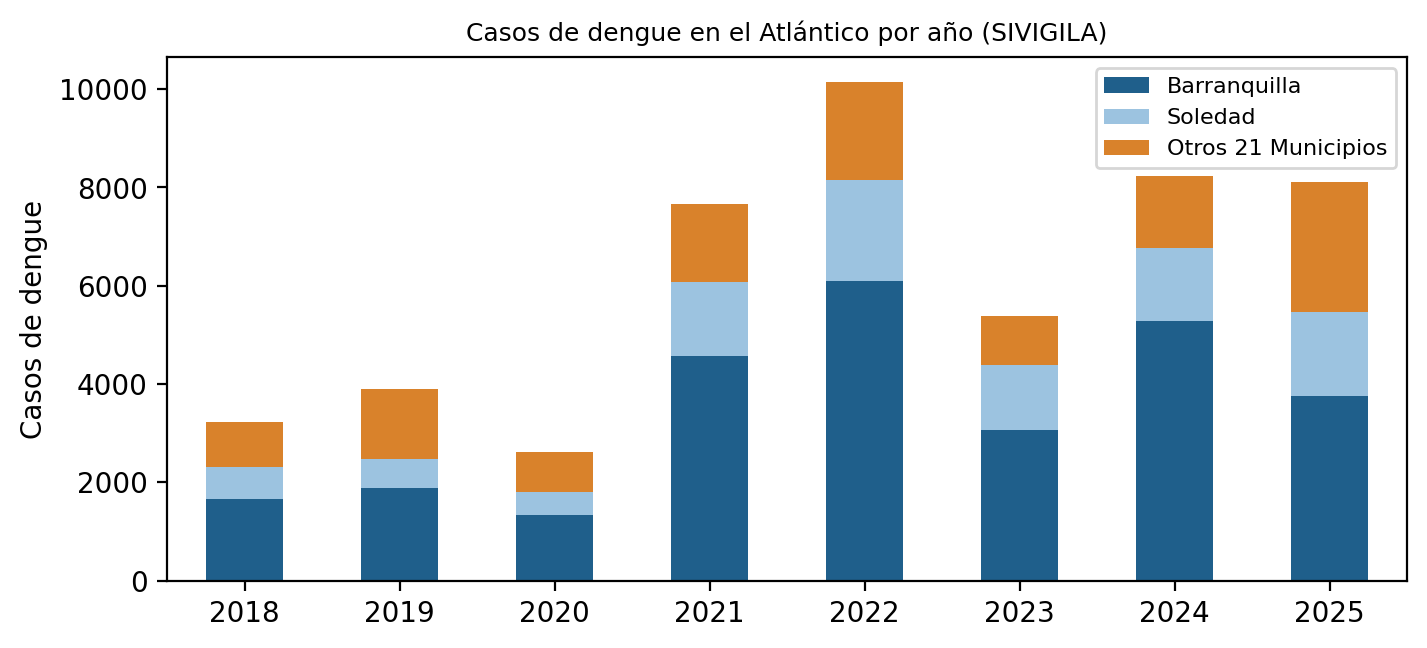
\includegraphics[width=0.85\textwidth]{figuras/casos_por_anio.png}
\caption{Casos anuales de dengue en el Atlántico, 2018--2025. Fuente: SIVIGILA.}
\label{fig:anios}
\end{figure}

\begin{figure}[H]
\centering
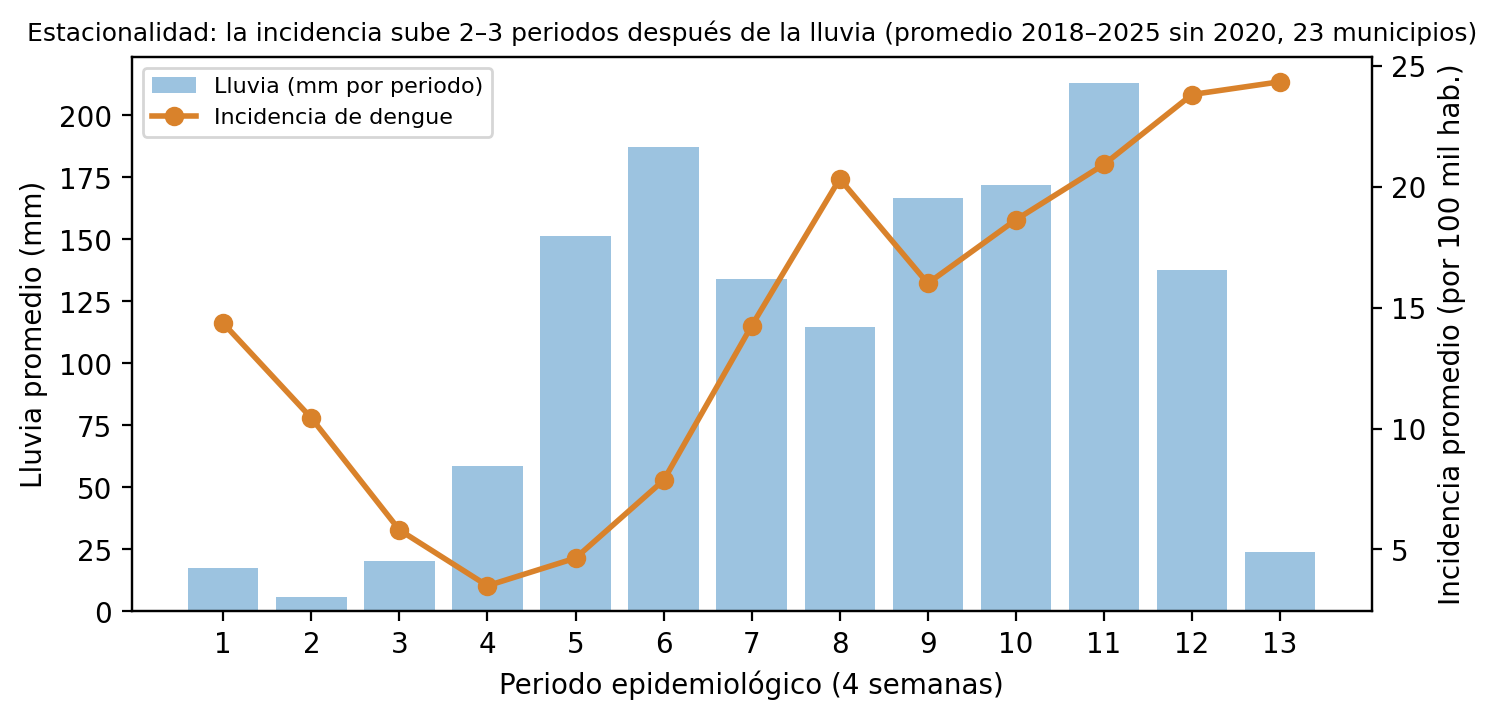
\includegraphics[width=0.88\textwidth]{figuras/estacionalidad.png}
\caption{Lluvia (barras) e incidencia de dengue (línea) promedio por periodo epidemiológico, 2018--2025 sin 2020. La incidencia sube dos o tres periodos después de la lluvia.}
\label{fig:estacion}
\end{figure}

\subsection{La estructura del grafo}
La Figura~\ref{fig:grafo} y la Tabla~\ref{tab:centralidad} muestran el resultado más interesante del grafo: los municipios más centrales \textbf{no} son los que más casos tienen. Barranquilla concentra el 56\,\% de los casos, pero tiene intermediación normalizada de apenas 0,010, porque está en el borde norte del departamento. Los puentes son Sabanalarga (0,370) y Baranoa (0,339), que conectan el área metropolitana con el centro y el sur. Un contagio que salga de Barranquilla hacia el sur tiene que pasar, en términos de vecindad, por ellos.

\begin{figure}[H]
\centering
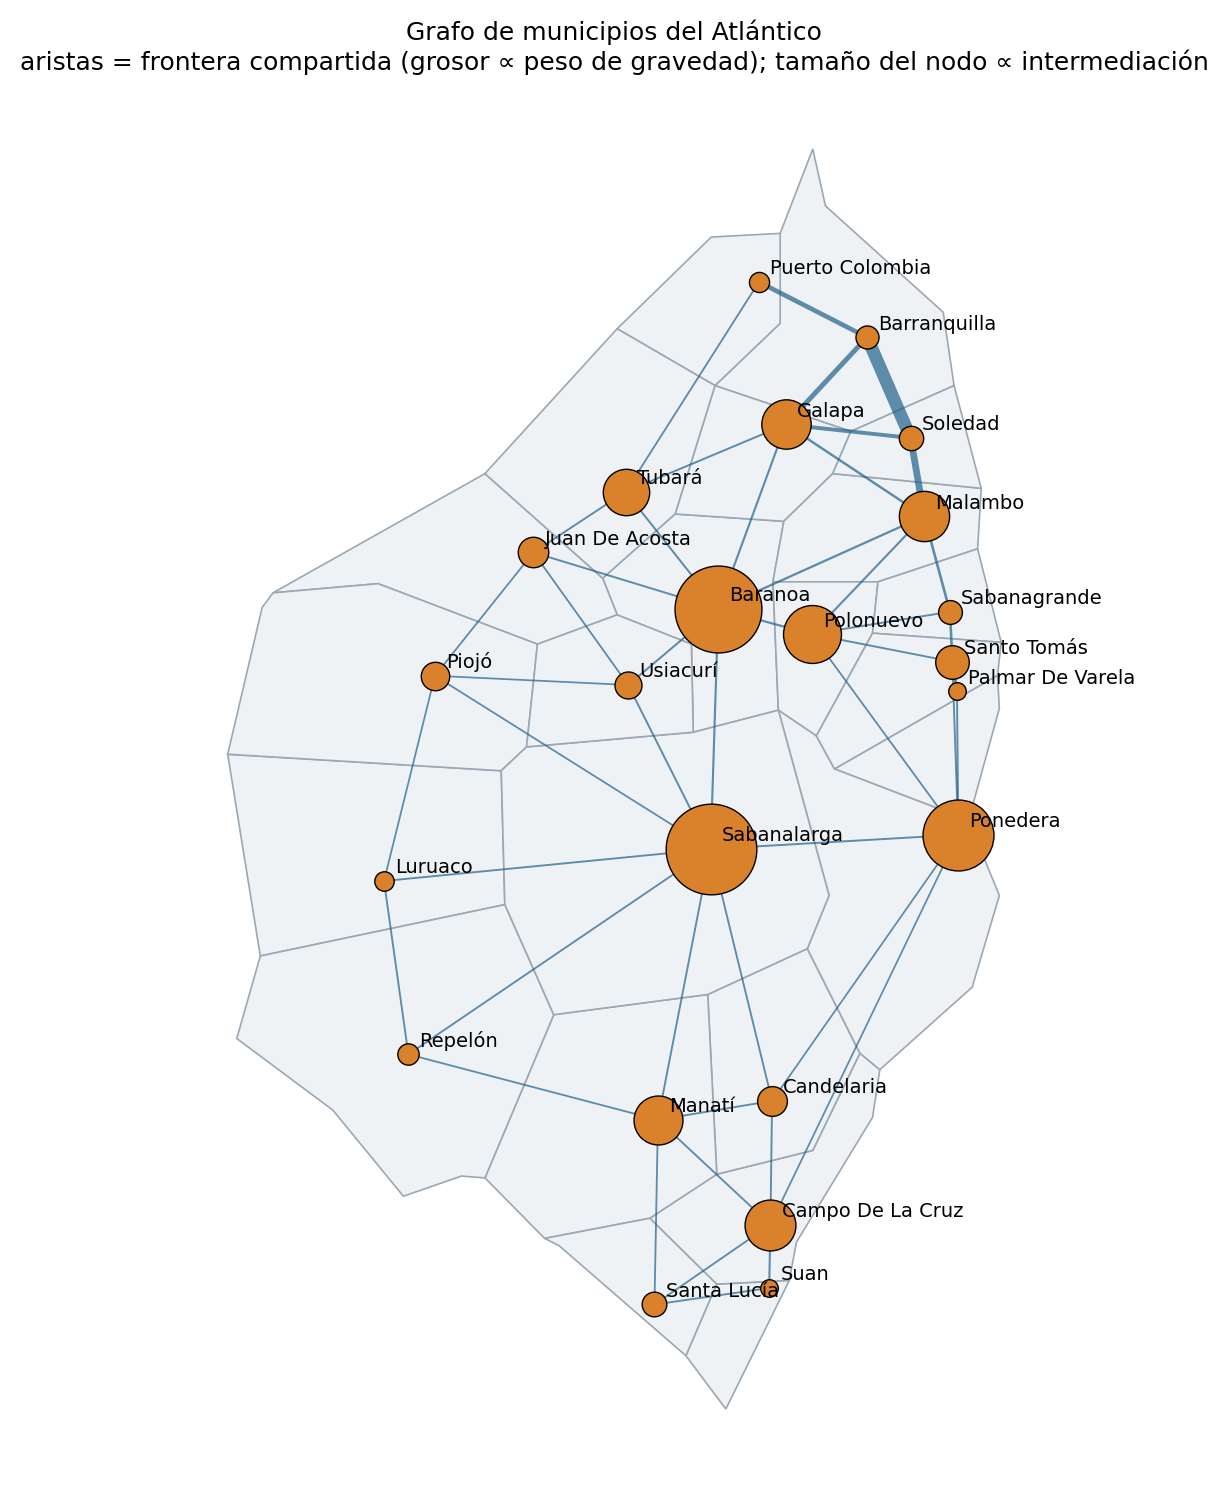
\includegraphics[width=0.62\textwidth]{figuras/grafo_atlantico.png}
\caption{Grafo de los 23 municipios. Las aristas unen municipios con frontera compartida, su grosor es proporcional al peso de gravedad y el tamaño de cada nodo es proporcional a su intermediación.}
\label{fig:grafo}
\end{figure}

\begin{table}[H]
\centering\small
\caption{Municipios con mayor intermediación, y Barranquilla y Soledad como referencia.}
\label{tab:centralidad}
\begin{tabular}{@{}lrrrr@{}}
\toprule
Municipio & Grado & Cercanía & Intermediación (norm.) & Casos 2018--2025 \\
\midrule
Sabanalarga & 8 & 0,537 & 0,370 & 1.629 \\
Baranoa & 7 & 0,524 & 0,339 & 1.438 \\
Ponedera & 6 & 0,478 & 0,221 & 333 \\
Polonuevo & 5 & 0,468 & 0,142 & 651 \\
Campo de la Cruz & 5 & 0,373 & 0,107 & 255 \\
\midrule
Soledad & 3 & 0,333 & 0,013 & 9.824 \\
Barranquilla & 3 & 0,301 & 0,010 & 27.616 \\
\bottomrule
\end{tabular}
\end{table}

\noindent Además, la presión de los vecinos tiene correlación de Spearman de 0,45 con la incidencia del periodo siguiente, y de 0,18 una vez se controla por la incidencia del propio municipio. Es decir, contiene algo de información que el municipio por sí solo no tiene.

\subsection{Comparación de modelos}
La Tabla~\ref{tab:modelos} y la Figura~\ref{fig:modelos} resumen los resultados en el año de prueba, 2025.

\begin{table}[H]
\centering\small
\caption{Resultados en el conjunto de prueba (2025, 299 filas, 100 brotes). Para la red: media $\pm$ desviación estándar en 20 semillas.}
\label{tab:modelos}
\begin{tabular}{@{}lccccc@{}}
\toprule
Modelo & Sensibilidad & Precisión & $F_2$ & AUC-ROC & AUC-PR \\
\midrule
Persistencia & 0,68 & \textbf{0,72} & 0,69 & 0,77 & 0,59 \\
Logística sin grafo & 0,85 & 0,52 & 0,75 & \textbf{0,84} & \textbf{0,75} \\
Logística con grafo & 0,86 & 0,50 & 0,75 & \textbf{0,84} & \textbf{0,75} \\
Red sin grafo & \textbf{0,88} $\pm$ 0,05 & 0,52 $\pm$ 0,04 & \textbf{0,77} $\pm$ 0,02 & \textbf{0,84} $\pm$ 0,01 & 0,72 $\pm$ 0,03 \\
Red con grafo & \textbf{0,88} $\pm$ 0,06 & 0,51 $\pm$ 0,05 & \textbf{0,77} $\pm$ 0,02 & 0,83 $\pm$ 0,01 & 0,72 $\pm$ 0,03 \\
\bottomrule
\end{tabular}
\end{table}

\begin{figure}[H]
\centering
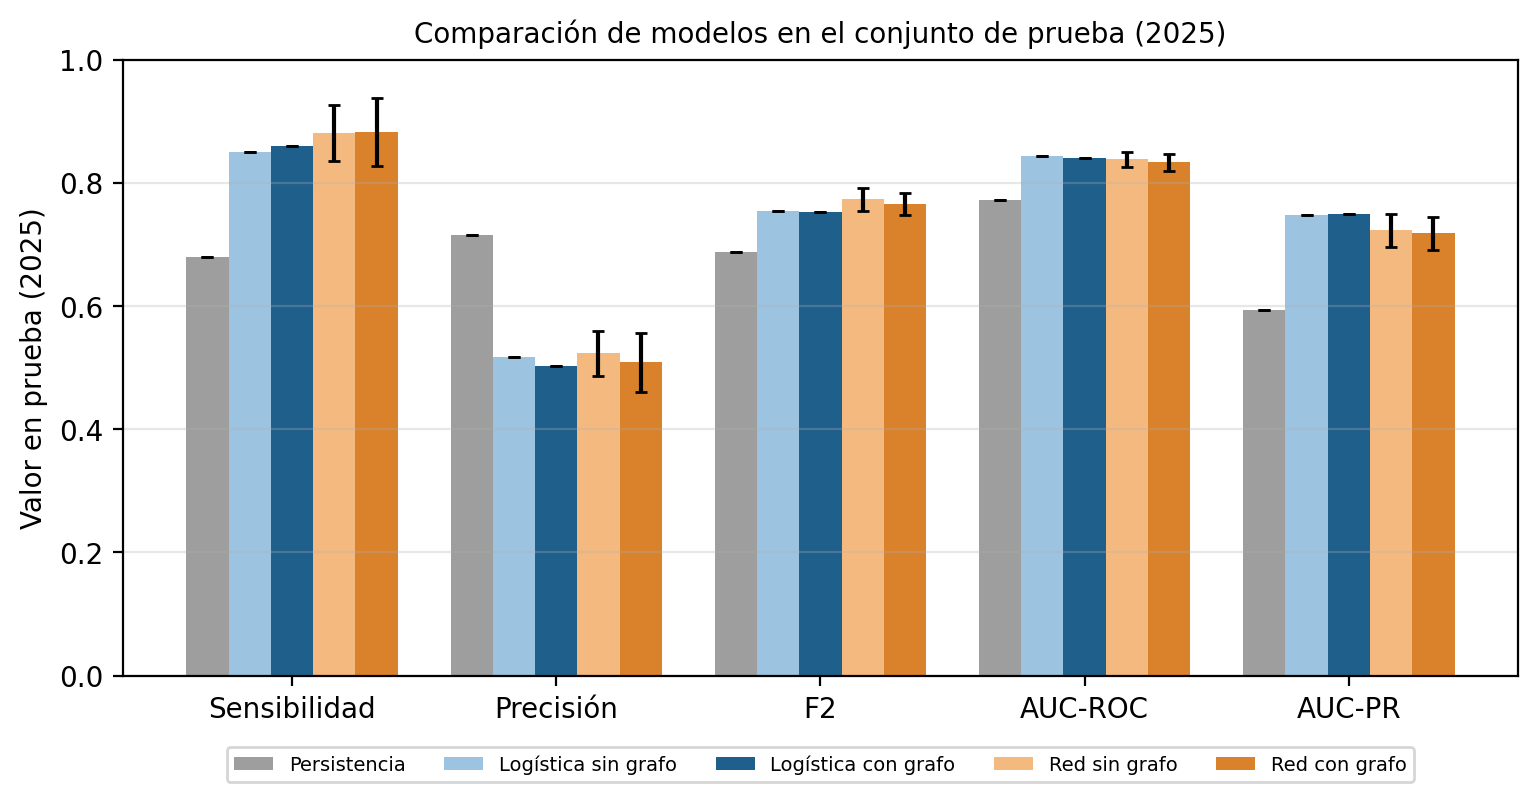
\includegraphics[width=0.9\textwidth]{figuras/metricas_modelos.png}
\caption{Métricas en el conjunto de prueba (2025). Las barras de error de la red son la desviación estándar en 20 semillas.}
\label{fig:modelos}
\end{figure}

\noindent Las conclusiones son tres:
\begin{enumerate}[label=\arabic*.]
  \item \textbf{Los modelos aprendidos superan a la persistencia.} Detectan entre el 85 y el 88\,\% de los brotes, frente al 68\,\%, y tienen mejor AUC. El costo es más falsas alarmas: la precisión baja de 0,72 a cerca de 0,50, algo esperable cuando el umbral se elige privilegiando la sensibilidad. En términos prácticos, por cada brote real se fumigaría también un municipio que no lo iba a tener.
  \item \textbf{La red no supera a la regresión logística.} Con unas 1.400 filas de entrenamiento no hay datos suficientes para que la red aproveche relaciones no lineales. Las dos son equivalentes dentro de la variabilidad entre semillas.
  \item \textbf{La presión de los vecinos no mejora la predicción.} La diferencia entre la red con grafo y la red sin grafo es de $-0{,}005\pm0{,}031$ en AUC-PR, $-0{,}006\pm0{,}016$ en AUC-ROC y $-0{,}007\pm0{,}027$ en $F_2$; la versión con grafo solo gana en 7 de 20 semillas. Se evaluó también la hipótesis de que el grafo ayudaría en los municipios con pocos datos, pero tampoco se confirmó (Tabla~\ref{tab:grupos}).
\end{enumerate}

\begin{table}[H]
\centering\small
\caption{AUC en prueba (2025) por tipo de municipio. ``Densos'': los seis municipios con casos en casi todos los periodos.}
\label{tab:grupos}
\begin{tabular}{@{}lcccc@{}}
\toprule
 & \multicolumn{2}{c}{AUC-ROC} & \multicolumn{2}{c}{AUC-PR} \\
Grupo & sin grafo & con grafo & sin grafo & con grafo \\
\midrule
6 municipios densos (78 filas) & 0,893 & 0,887 & 0,879 & 0,871 \\
17 municipios escasos (221 filas) & 0,833 & 0,827 & 0,666 & 0,665 \\
\bottomrule
\end{tabular}
\end{table}

\noindent\textbf{¿Por qué el grafo no ayuda a predecir?} Hay tres explicaciones compatibles con los datos. Primera: la incidencia propia ya resume casi toda la información; la señal adicional de los vecinos (correlación parcial de 0,18) es real, pero pequeña para cambiar una decisión binaria. Segunda: en el Atlántico los brotes son casi simultáneos, porque todos los municipios comparten el mismo clima y la misma temporada, así que saber que el vecino está en brote dice poco que la lluvia y el periodo del año no digan ya. Tercera: el grafo solo incluye vecinos dentro del departamento.

\subsection{Donde el grafo sí aporta: la prioridad de fumigación}
Predecir no es lo mismo que decidir. Si dos municipios tienen riesgo parecido, conviene fumigar primero el que más rutas de contagio corta. Por eso se define
\begin{equation}
  \text{Prioridad}(v) = \hat P(\text{brote}_v) \times \left(1 + \frac{B(v)}{\max_u B(u)}\right).
\end{equation}
La centralidad puede, como mucho, duplicar la prioridad, y el riesgo propio sigue dominando. Se suma 1 para que un municipio de alto riesgo con intermediación nula no quede en cero. Para el pronóstico se reentrenó la red con grafo con todos los años etiquetados excepto 2020 (20 semillas), con el umbral promedio de validación, $\tau=0{,}44$. El resultado para el periodo 1 de 2026 aparece en la Figura~\ref{fig:prioridad} y la Tabla~\ref{tab:prioridad}.

\begin{table}[H]
\centering\small
\caption{Pronóstico y prioridad para el periodo 1 de 2026: los cinco primeros puestos.}
\label{tab:prioridad}
\begin{tabular}{@{}clccc@{}}
\toprule
Puesto & Municipio & $\hat P$(brote) & Intermediación relativa & Prioridad \\
\midrule
1 & Sabanalarga & 0,71 & 1,00 & 1,42 \\
2 & Ponedera & 0,82 & 0,60 & 1,31 \\
3 & Baranoa & 0,65 & 0,92 & 1,25 \\
4 & Polonuevo & 0,90 & 0,39 & 1,25 \\
5 & Galapa & 0,93 & 0,27 & 1,18 \\
\bottomrule
\end{tabular}
\end{table}

\begin{figure}[H]
\centering
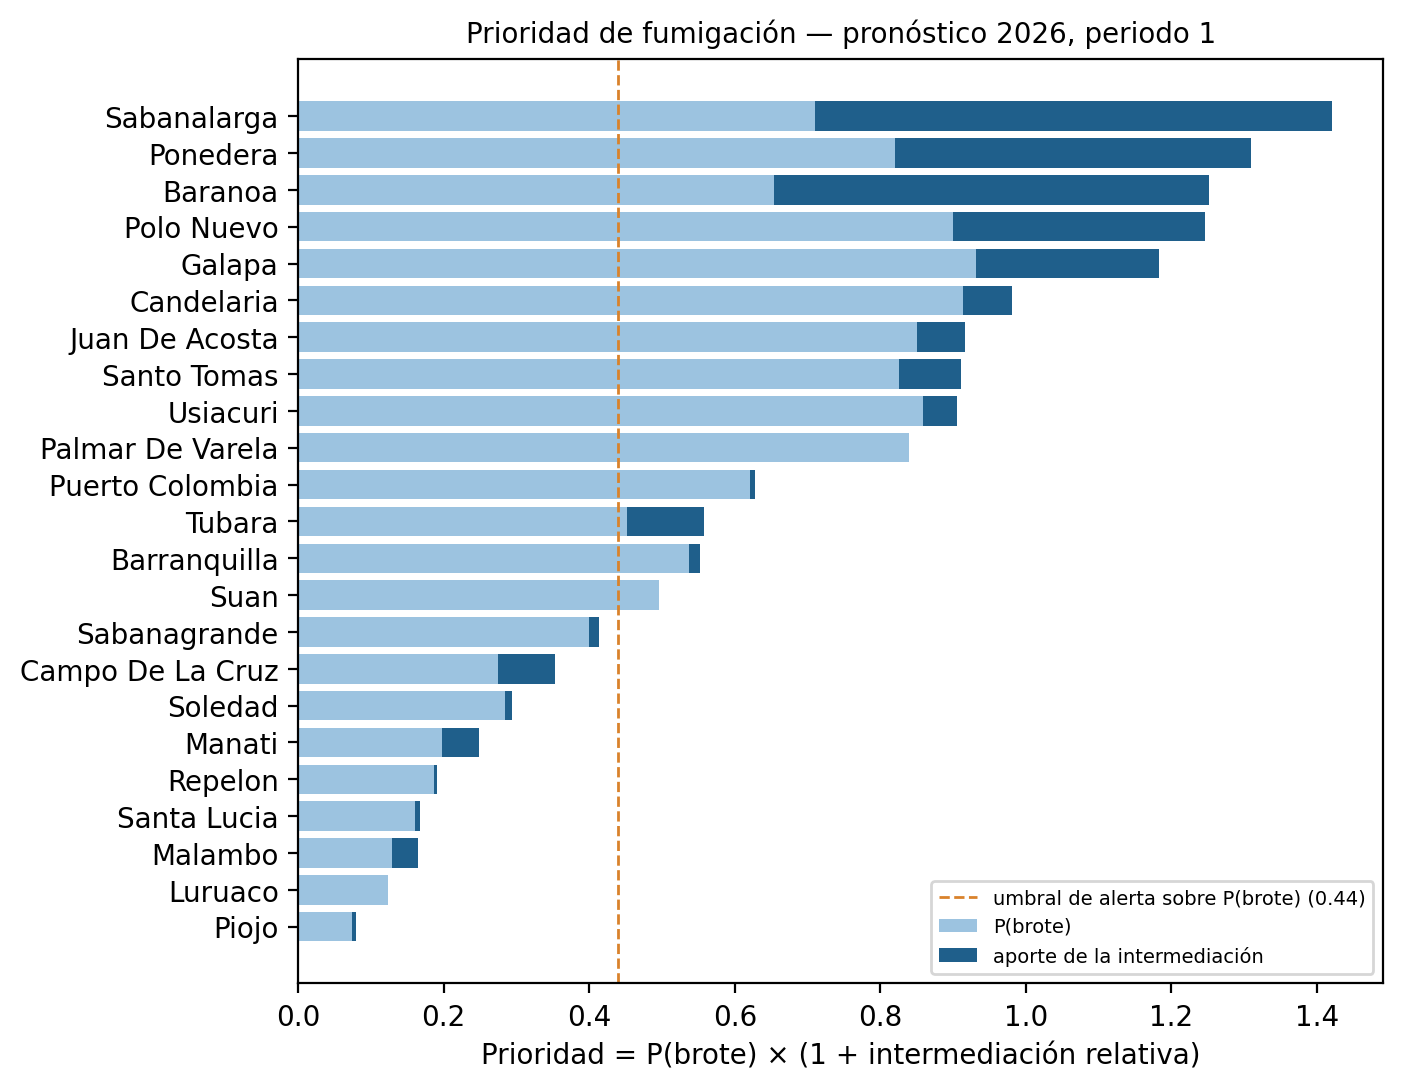
\includegraphics[width=0.66\textwidth]{figuras/prioridad_2026_p1.png}
\caption{Prioridad de fumigación para el periodo 1 de 2026. Azul claro: probabilidad de brote. Azul oscuro: aporte de la intermediación.}
\label{fig:prioridad}
\end{figure}

\noindent Catorce de los 23 municipios quedan en alerta, lo que es coherente con el pico estacional de diciembre a enero y con un 2025 de muchos brotes. Sabanalarga y Baranoa suben al primer y tercer puesto por ser puentes del grafo, aunque su probabilidad no es la más alta; Galapa y Candelaria tienen la probabilidad más alta (0,93 y 0,91). Este pronóstico todavía no se puede verificar, porque el SIVIGILA publica sus microdatos con varios meses de retraso.

% ======================== 5. CONCLUSIONES ===========================
\section{Conclusiones y limitaciones}

\paragraph{Conclusiones.}
\begin{enumerate}[label=\arabic*.]
  \item Es posible anticipar con un periodo de antelación la mayoría de los brotes de dengue en el Atlántico con datos públicos: el 88\,\% en 2025, frente al 68\,\% de la regla de persistencia.
  \item La lluvia de hace dos o tres periodos, es decir, de ocho a doce semanas, es la variable climática más relacionada con los casos.
  \item Una red neuronal pequeña no supera a una regresión logística con estos datos. Con poco más de mil filas, el modelo más simple es igual de bueno y más fácil de explicar.
  \item El grafo de vecindad \textbf{no} mejoró la predicción, pero sí aportó a la \textbf{decisión}: la intermediación muestra que los puentes del contagio son Sabanalarga y Baranoa, no Barranquilla. Un ranking de fumigación que combine riesgo y centralidad prioriza esos municipios.
  \item Los algoritmos de grafos implementados por el grupo (BFS y Brandes) coinciden exactamente con los cálculos a mano y con NetworkX.
\end{enumerate}

\paragraph{Limitaciones.}
\begin{itemize}
  \item Los datos de 2020 y 2021 están afectados por la pandemia. 2020 se excluyó; en 2021 se asumió que el brote de fin de año es real.
  \item Se usan casos notificados, que dependen de que las personas consulten. Un 6\,\% de los casos son probables y no confirmados.
  \item El clima viene de un modelo numérico de 9\,km, no de estaciones, así que se usaron anomalías y no milímetros absolutos.
  \item La definición de brote depende de solo cinco años de entrenamiento por municipio y periodo.
  \item El grafo ignora a los municipios de Magdalena y Bolívar que limitan con el departamento, y aproxima la movilidad con un modelo de gravedad en lugar de datos reales de viajes.
  \item La prioridad propuesta no se ha validado contra intervenciones reales, y el pronóstico de 2026 todavía no se puede verificar.
\end{itemize}

\paragraph{Trabajo futuro.} Usar datos reales de movilidad, como rutas de transporte intermunicipal, para los pesos del grafo; incluir los municipios vecinos de otros departamentos; y evaluar la prioridad con una simulación de contagio sobre el grafo (modelo SIR en red), comparando qué ocurre al ``retirar'' los municipios de mayor prioridad.

% ======================== REFERENCIAS (APA 7) =======================
\newpage
\begin{thebibliography}{99}
\setlength{\itemsep}{3pt}\small
\setlength{\leftskip}{1.27cm}\setlength{\itemindent}{-1.27cm}

\bibitem[Brandes(2001)]{brandes2001}
Brandes, U. (2001). A faster algorithm for betweenness centrality. \emph{Journal of Mathematical Sociology, 25}(2), 163--177. \url{https://doi.org/10.1080/0022250X.2001.9990249}

\bibitem[Departamento Administrativo Nacional de Estadística {[DANE]}(2018)]{dane_mgn}
Departamento Administrativo Nacional de Estadística [DANE]. (2018). \emph{Marco Geoestadístico Nacional: límites municipales} [Conjunto de datos]. \url{https://geoportal.dane.gov.co/}

\bibitem[DANE(2025a)]{dane_pob}
Departamento Administrativo Nacional de Estadística [DANE]. (2025a). \emph{Serie municipal de población por área, para el periodo 2018--2042} [Conjunto de datos]. \url{https://www.dane.gov.co/index.php/estadisticas-por-tema/demografia-y-poblacion/proyecciones-de-poblacion}

\bibitem[DANE(2025b)]{dane_divipola}
Departamento Administrativo Nacional de Estadística [DANE]. (2025b). \emph{DIVIPOLA: códigos municipios} [Conjunto de datos]. Datos Abiertos Colombia. \url{https://www.datos.gov.co/resource/gdxc-w37w}

\bibitem[El Tiempo(2024)]{eltiempo2024}
El Tiempo. (2024). \emph{Atlántico: 1.518 casos de dengue se registran en el departamento por temporada de lluvias}. \url{https://www.eltiempo.com/colombia/barranquilla/atlantico-mas-de-4-000-casos-probables-registrados-en-el-departamento-por-temporada-de-lluvias-3383977}

\bibitem[El Universal(2026)]{eluniversal2026}
El Universal. (2026, 4 de junio). \emph{Por aumento de casos, intensifican acciones contra el dengue en el Atlántico}. \url{https://www.eluniversal.com.co/regional/atlantico/2026/06/04/por-aumento-de-casos-intensifica-acciones-contra-el-dengue-en-el-atlantico/}

\bibitem[Freeman(1977)]{freeman1977}
Freeman, L. C. (1977). A set of measures of centrality based on betweenness. \emph{Sociometry, 40}(1), 35--41. \url{https://doi.org/10.2307/3033543}

\bibitem[Goodfellow et~al.(2016)]{goodfellow2016}
Goodfellow, I., Bengio, Y., \& Courville, A. (2016). \emph{Deep learning}. MIT Press.

\bibitem[Hagberg et~al.(2008)]{hagberg2008}
Hagberg, A. A., Schult, D. A., \& Swart, P. J. (2008). Exploring network structure, dynamics, and function using NetworkX. En G. Varoquaux, T. Vaught, \& J. Millman (Eds.), \emph{Proceedings of the 7th Python in Science Conference} (pp. 11--15).

\bibitem[Instituto Nacional de Salud {[INS]}(2026)]{sivigila}
Instituto Nacional de Salud [INS]. (2026). \emph{Portal SIVIGILA 4.0: búsqueda de microdatos, evento Dengue (210), 2018--2025} [Conjunto de datos]. \url{https://portalsivigila.ins.gov.co/Paginas/Buscador.aspx}

\bibitem[Morin et~al.(2013)]{morin2013}
Morin, C. W., Comrie, A. C., \& Ernst, K. (2013). Climate and dengue transmission: Evidence and implications. \emph{Environmental Health Perspectives, 121}(11--12), 1264--1272. \url{https://doi.org/10.1289/ehp.1306556}

\bibitem[Organización Mundial de la Salud {[OMS]}(s.~f.)]{oms_dengue}
Organización Mundial de la Salud [OMS]. (s.~f.). \emph{Dengue and severe dengue} [Nota descriptiva]. Recuperado el 8 de noviembre de 2026, de \url{https://www.who.int/news-room/fact-sheets/detail/dengue-and-severe-dengue}

\bibitem[Pedregosa et~al.(2011)]{pedregosa2011}
Pedregosa, F., Varoquaux, G., Gramfort, A., Michel, V., Thirion, B., Grisel, O., Blondel, M., Prettenhofer, P., Weiss, R., Dubourg, V., Vanderplas, J., Passos, A., Cournapeau, D., Brucher, M., Perrot, M., \& Duchesnay, É. (2011). Scikit-learn: Machine learning in Python. \emph{Journal of Machine Learning Research, 12}, 2825--2830.

\bibitem[Xia et~al.(2004)]{xia2004}
Xia, Y., Bjørnstad, O. N., \& Grenfell, B. T. (2004). Measles metapopulation dynamics: A gravity model for epidemiological coupling and dynamics. \emph{The American Naturalist, 164}(2), 267--281. \url{https://doi.org/10.1086/422341}

\bibitem[Zippenfenig(2023)]{openmeteo}
Zippenfenig, P. (2023). \emph{Open-Meteo.com Weather API} [Software]. Zenodo. \url{https://doi.org/10.5281/zenodo.7970649}

\end{thebibliography}

% ======================== APÉNDICE ==================================
\appendix
\section{Reproducibilidad}
El código, los datos y las instrucciones están en la carpeta del proyecto. Para reproducir todos los resultados:
\begin{verbatim}
pip install -r requirements.txt
python src/01_casos.py
python src/02_poblacion_clima.py
python src/03_grafo.py
python src/04_dataset.py
python src/05_modelo.py        # ~20 s
python src/06_prioridad.py
python src/07_figuras_descriptivas.py
python tests/test_semana_epi.py
python tests/test_grafo.py
python tests/test_dataset.py
\end{verbatim}
El registro completo de decisiones está en \texttt{BITACORA.md}.

\end{document}
